\subsection{Was ist \acs{csv}?}
\acf{csv} ist ein systemunabhängiges Format für Klartextdateien. \acs{csv} Dateien dienen zum Speichern und Übertragen von strukturierten Daten, hauptsächlich Tabellen oder Listen, wobei durch die Verkettung von mehreren \acs{csv} Dateien oder mithilfe von zusätzlichen Regeln auch verschachtelte Objekte gespeichert werden können. Die hauptsächlichen Anwendungsbereiche von \acs{csv} Dateien sind zum Importieren und Exportieren von Daten aus Datenbanken oder die Migration von Tabellendaten zwischen Programmen. \cite{FuchsMediaSolutions:o.J.}

Die erste Verwendung des Datenformates geht auf 1972 zurück, wo es vom IBM FORTRAN IV (H Extended) Compiler \cite{IBM:1972} unterstützt wurde. Trotz der langen Existenz gibt es gegenwärtig für \acs{csv} keine formelle Spezifikation. Mit dem \acs{rfc} 4180 \cite{Shafranovich:2005} aus dem Jahre 2005 existiert ein erster Versuch einer inoffiziellen Definition, welche mittlerweile weit verbreitet ist. Durch dieses Dokument wird das \acf{mime} "text/csv"\ für das \acs{csv} Format registriert. Es folgen die wesentlichen Merkmale aus der Definition des \acs{rfc} 4180:

\begin{enumerate}{}
	
	\item Jedem Datensatz steht eine Zeile zu, die mit einem Zeilenumbruch (\ac{crlf}) beendet wird. Ein Zeilenumbruch am Ende des letzten Datensatzes ist optional. \zB 
	\begin{lstlisting}
	aaa, bbb, ccc CRLF
	xxx, yyy, zzz CRLF
	\end{lstlisting}
	oder
	\begin{lstlisting}
	aaa, bbb, ccc CRLF
	xxx, yyy, zzz
	\end{lstlisting}
	
	\item Am Anfang eines \acs{csv} Dokumentes kann es eine Kopfzeile geben. Diese hat das Format eines normalen Datensatzes und beinhaltet Namen für die Spalten (Felder). Die Anzahl der Spalten sollte für Kopfzeile und Datensätze gleich sein. \zB
	\begin{lstlisting}
	spaltenname_1, spaltenname_2, spaltenname_3 CRLF
	aaa, bbb, ccc CRLF
	xxx, yyy, zzz CRLF
	\end{lstlisting}
	
	\item Sowohl in den Datensätzen als auch in der Kopfzeile kann es eine oder mehrere Spalten geben, die jeweils immer durch einen Beistrich (\acs{engl} comma) separiert werden. Am Ende einer Zeile bedarf es keines Beistrichs. Abstände sind Teil eines Feldes und müssen berücksichtigt werden. (Anmerkung: Auch wenn das eigentliche Format Beistriche für die Feldtrennung vorsieht, werden oft andere Zeichen wie \zB Strichpunkte (Semikolons) verwendet.)
	
	\item Jedes Feld kann in Anführungszeichen eingeschlossen sein und darf dann auch Beistriche, Zeilenumbrüche oder Anführungszeichen beinhaltet. \zB
	\begin{lstlisting}
	"aaa","b CRLF
	bb","ccc" CRLF
	xxx,yyy,zzz
	\end{lstlisting}
	
\end{enumerate}

Da es bei \acs{csv} keine festen Vorgaben beim Datenformat gibt, ist es die Verantwortung der Benutzer sich auf eine Formatierung zu einigen. Das führt oft zu Problemen bei Zeit- und Datumsangaben oder bei der Verwendung von Sonderzeichen. Eine weitere Hürde ist die fehlende explizite Angabe des verwendeten Zeichensatzes, womit \zB Umlaute fehlerhaft dargestellt werden können. \cite{FuchsMediaSolutions:o.J.}

\subsection{Was ist \acs{json}?}
\acf{json} wurde 2001 auf der "JSON.org"\ Website veröffentlicht und ist ein ressourcenschonendes Textformat zum Speichern von strukturierten Daten. Es ist so konzipiert, dass es sowohl für Menschen einfach zu lesen und schreiben als auch für Maschinen einfach zu parsen und generieren ist. \acs{json} stammt von JavaScript, ist aber programmiersprachenunabhängig und folgt vielen Konventionen der C-basierten Sprachen, was es gut für den Datenaustausch macht. \cite{json_org:o.J.} \cite{ECMA:2017} 

\acs{json} wird derzeit von zwei Spezifikation definiert, ECMA-404 \cite{ECMA:2017} und RFC 8259 \cite{Bray:2017}. Dabei ist das Ziel, dass sich nur die Beschreibung des Formats unterscheidet, aber die \acs{json} Syntax beider Spezifikationen ident ist. Folgend wird sich auf die Beschreibung der offiziellen \url{JSON.org} Website \cite{json_org:o.J.} und somit auf ECMA-404 \cite{ECMA:2017} bezogen.

Die zwei wichtigsten Strukturen auf denen \acs{json} aufbaut sind Name/Wert (\engl Key/Value) Paare und geordnete Listen von Werten. Dabei unterstützt \acs{json} sehr verschachtelte Strukturen. Um diese darzustellen, werden in der Syntax folgende Zeichen benötigt:
\begin{itemize}
	 \item Beistriche \lstinline|,|
	 \item Doppelpunkte \lstinline|:|
	 \item Eckige Klammern \lstinline|[ ]|
	 \item Geschwungene Klammern \lstinline|{ }|
\end{itemize}


Mithilfe dieser Syntax, kann man in \acs{json} folgende Strukturen umsetzen:
\begin{itemize}
	\item \textbf{Values} (\dt Werte) sind, entweder vom Typ "'object"', "'string"', "'array"', "'number"' oder haben den Wert "'false"', "'true"', oder "'null"' (siehe Abb.~\ref{fig:json_value}).
	\begin{figure}[H]
		\centering
		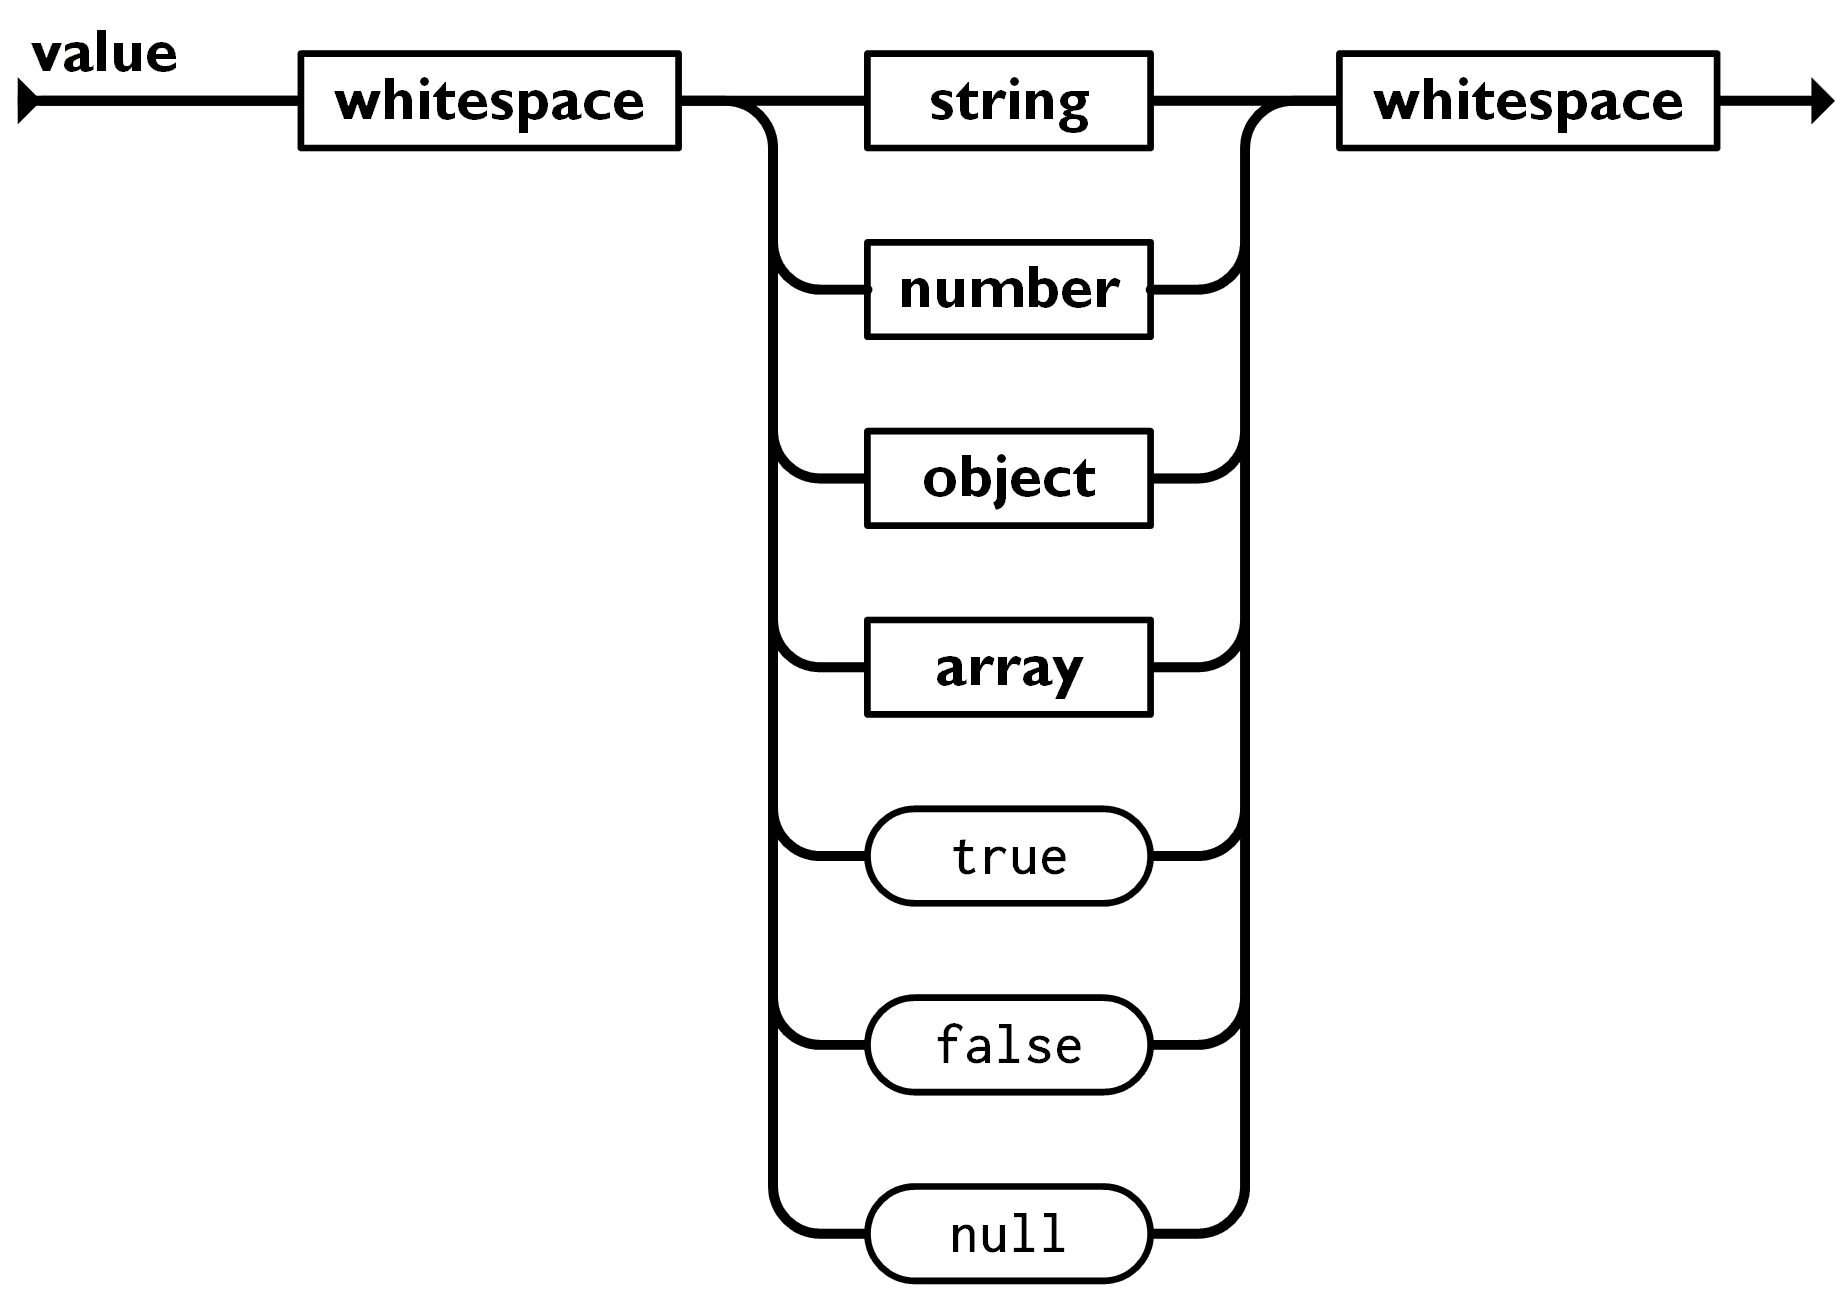
\includegraphics[width=10cm]{JSON_value}
		\caption[JSON Wert]{\acs{json} Value (Quelle: \url{https://www.json.org/img/value.png})  \label{fig:json_value}}
	\end{figure}
	
	\item \textbf{Objects} (\dt Objekte) sind ungeordnete Listen von beliebig vielen Name/Wert Paaren. Ein Name/Wert Paar besteht immer aus einem Namen, gefolgt von einem Doppelpunkt und dem zugehörigen Wert. Beistriche kommen zum Einsatz um Name/Wert Paare voneinander zu trennen. Ein Objekt wird immer von geschwungenen Klammern umschlossen. Der Aufbau eines \acs{json} Objekts ist in Abb.~\ref{fig:json_object} zu sehen.
	
	\begin{figure}[H]
		\centering
		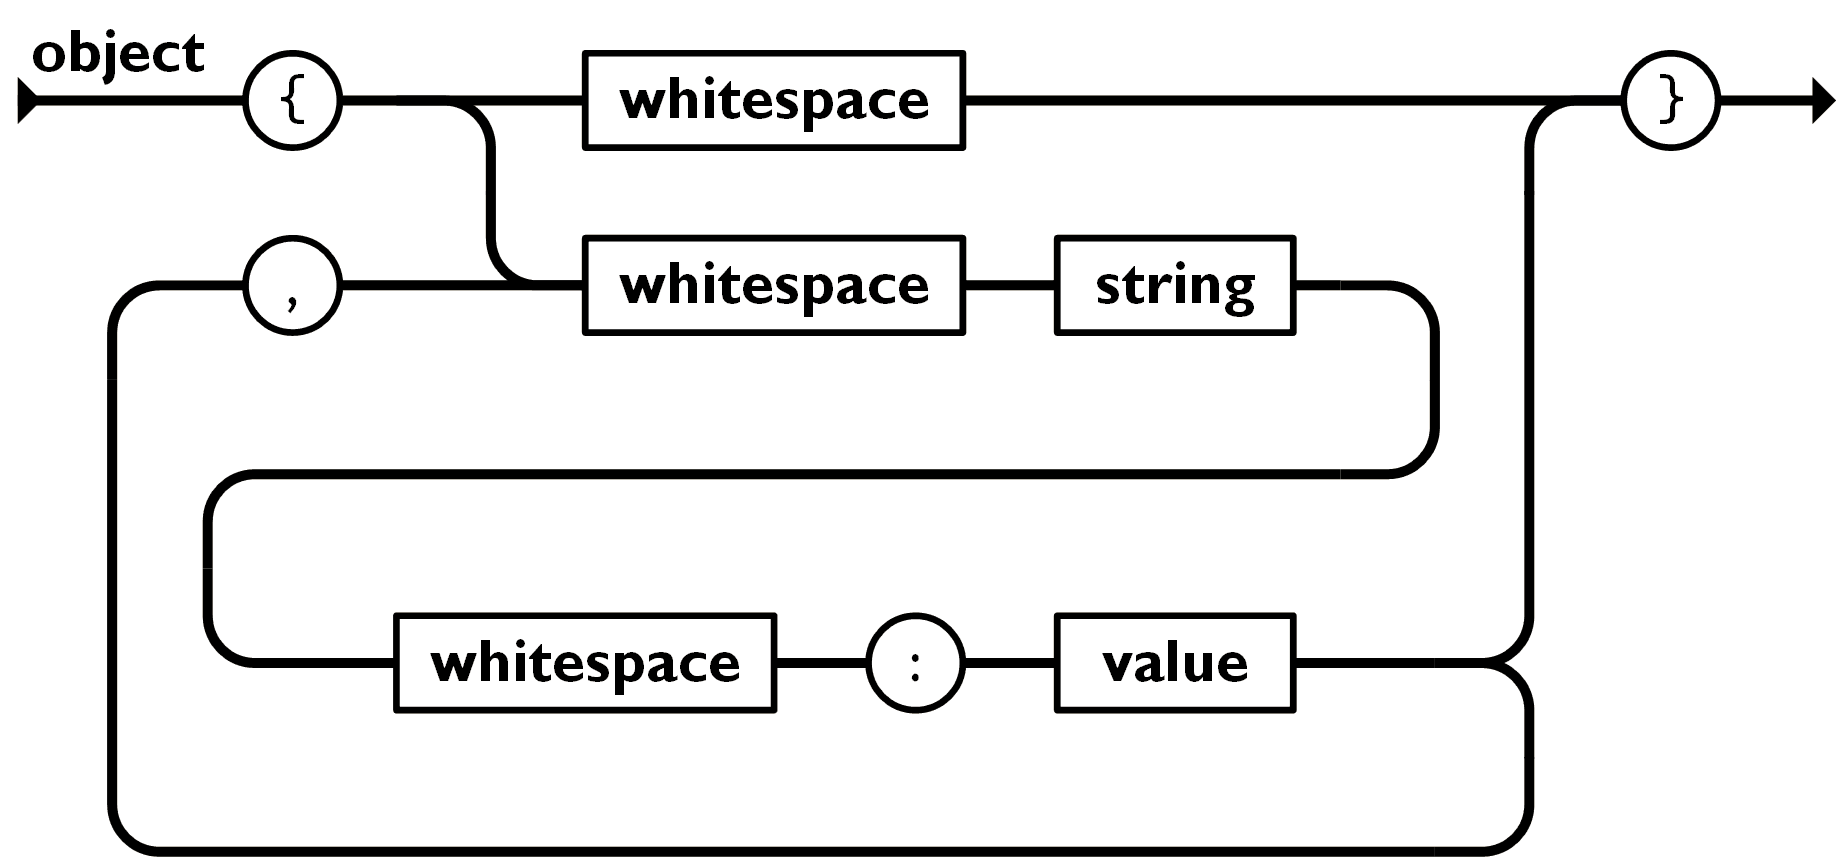
\includegraphics[width=10cm]{JSON_object}
		\caption[JSON Objekt]{\acs{json} Object (Quelle: \url{https://www.json.org/img/object.png})  \label{fig:json_object}}
	\end{figure}
	
	\item \textbf{Arrays} sind geordnete Listen von Werten. Dabei werden Beistriche verwendet, um die Werte voneinander zu trennen. Ein Array wird immer von eckigen Klammern umschlossen. Der Aufbau eines Arrays ist in Abb.~\ref{fig:json_array} zu sehen.
	
	\begin{figure}[H]
		\centering
		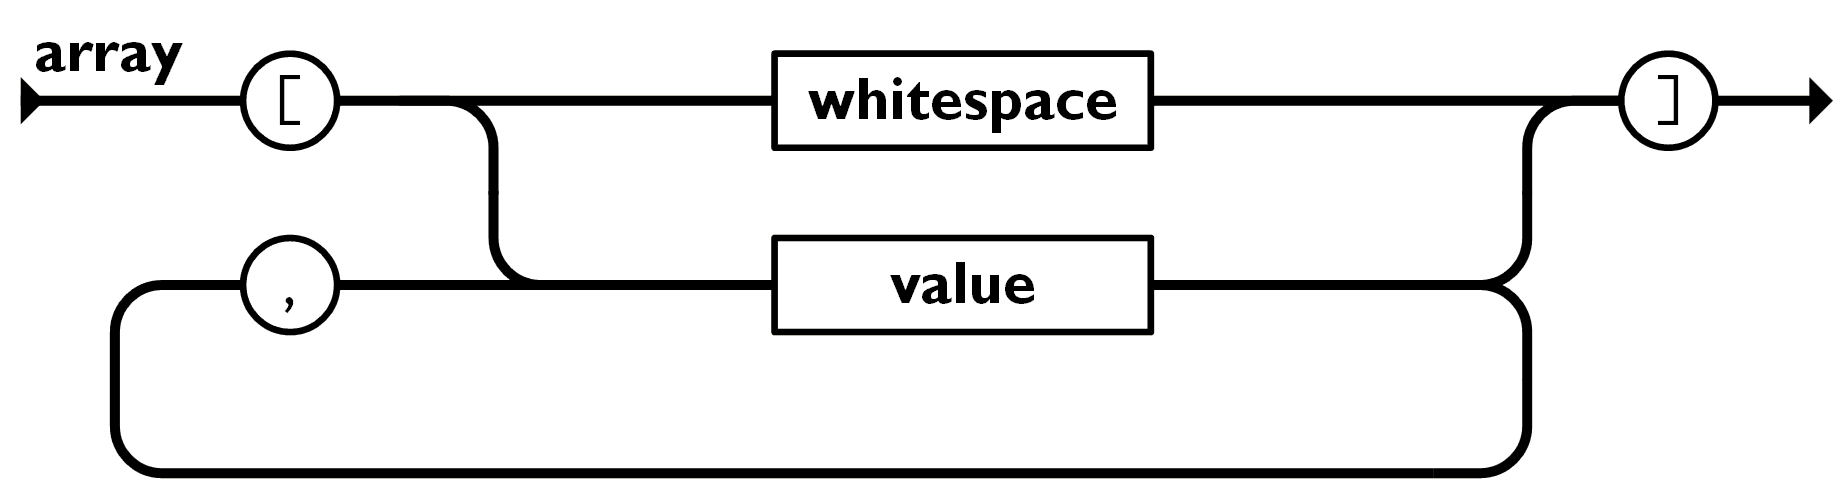
\includegraphics[width=10cm]{JSON_array}
		\caption[JSON Array]{\acs{json} Array (Quelle: \url{https://www.json.org/img/array.png})  \label{fig:json_array}}
	\end{figure}
	
	\item \textbf{Strings} sind Zeichenketten. Sie können entweder leer sein, d. h. aus keinen Zeichen bestehen oder mehrere Unicode Zeichen enthalten. Eine Zeichenkette wird immer von Anführungszeichen umschlossen. Sie kann auch besondere Escapesequenzen beinhalten, die besondere Bedeutungen haben. Diese werden mit einem Backslash aufgerufen, wie \zB "\textbackslash n",\ "\textbackslash t"\ oder "\textbackslash r".
	
	\item \textbf{Numbers} (\dt Zahlen) sind numerische Werte, die aus einer oder mehreren dezimalen Ziffern bestehen. Sie können also keine Werte wie \zB "'Infinity"' oder "'NaN"' annehmen. Außerdem werden sie nie von Anführungszeichen umschlossen. 
	
\end{itemize}

\subsection{\acs{json} und \acs{csv} - Vergleich und Selektion}
\cite{SQLizer:2017}
